\chapter{Asking Billionaires How They Got RICH!}

We begin, not with a theorem on a blackboard, but with wealth in its outward form: the G-Wagon, the Ferrari, the quick answer about what one does, and the abrupt mention of annual numbers. The lecture then performs a more serious move. It turns these surfaces into a field of inquiry and asks what is actually being sampled: persistence, cash discipline, leverage, delegation, retained earnings, working capital, and the business logic that sits underneath a high-income profession. What follows is therefore best read as a sequence of operating principles extracted from short encounters, with the arithmetic of business finance slowly becoming more explicit as the lecture proceeds.

\section{Houston as a Search Space}

The opening montage is deliberately theatrical. It gives us a football owner, a doctor, and rapid dollar figures before we know how any of them fit together. Then the lecture widens the frame and names the terrain: Houston, and more specifically River Oaks, as a place where the concentration of wealth is large enough that the street interview can serve as a crude sampling device.

The transcript states that Houston is the eighth city in the world in millionaire concentration. Whether or not that ranking is independently verified elsewhere is not the point of the chapter; within the lecture it functions as a premise for the search:
\begin{equation}
\operatorname{rank}_{\text{millionaire-city}}(\text{Houston}) = 8.
\end{equation}
The real narrative function of the opening is to tell us that luxury objects are not yet the lesson. They are merely markers that help the speaker locate people whose business decisions may be worth interrogating.

This matters for the tone of the notes. We should not read the cars as evidence of a theory of wealth. We should read them as a selection rule: first find the visible signal, then test whether there is an operating logic beneath it.

\section{Refusal as Method}

Before the lecture gives us a developed theory, it gives us refusals. Several early approaches fail, and that is not incidental. The speaker keeps the friction in the edit because the first principle is methodological rather than financial: access is hard, and persistence begins before any explicit business content appears.

In the transcript, the host converts rejection into a rule of search. A no is not treated as terminal; it is treated as movement through the search space toward a yes. This should remain in the chapter because it is the lecture's first disciplined transition from spectacle to method.

The first small payoff comes in compressed form through the restaurant-owner exchange. The answers are brief, almost aphoristic, but they establish the earliest operating vocabulary:
\begin{itemize}
\item Be fearless.
\item Do not be afraid to fail.
\item A good product still sits underneath the scale story.
\end{itemize}
These are not yet developed into a full model, but they prepare the ground. The lecture is teaching us how to hear later answers. When a larger owner says ``never quit,'' we will need to ask what concrete machinery makes that principle survivable.

\section{The Texans Interview: Persistence at Larger Scale}

The lecture then repeats one of its opening hooks, but now in a fuller and more serious form. We meet the owner of the Houston Texans, and the scene immediately raises the stakes. The earlier teaser gave us the outward claim; this interview begins to connect wealth to prior business success, cash conservatism, leverage, and negotiation.

The central slogan here is simple: never quit. But the lecture does not leave the slogan floating. It asks how one enters a competitive field, what prior business made the next move possible, what advice came from mentors, and how one should negotiate.

\subsection{Question \& Answer}

\paragraph{Question.} What does persistence look like once the stakes are large?

\paragraph{Answer.} In this interview, persistence is not merely emotional stamina. It is persistence supported by earlier success in another business, by conserving cash, by tolerating leverage, and by refusing to negotiate from desperation. The speaker's short rule about negotiating --- that one should want the deal, but not want it too badly --- can be written in a minimal decision-theoretic form as
\begin{equation}
V_{\text{deal}} \geq V_{\text{walk}},
\end{equation}
where \(V_{\text{walk}}\) is the value of the outside option. If walking away is not live, then the bargaining stance collapses.

\begin{remark}
The lecture's phrase ``conserve your cash'' plays the same structural role. Opportunities do not arrive on a smooth schedule, and cash is what permits action when they do.
\end{remark}

This is why the host's recap immediately after the interview matters. He retells the conversation as a lesson about not quitting just before the breakthrough. In the notes we should preserve that recap, because it turns a vivid anecdote into portable doctrine and sets up the next, much denser interview.

\section{From Self-Employment to Organization}

The Ferrari interview is where the lecture ceases to be merely motivational and becomes organizational. The founder describes a labor-force management company and is asked about delegation, team-building, and the difference between working in the business and working on the business. This is the first point at which the lecture gives us a clean quantitative contrast.

\begin{definition}
In the vocabulary of this lecture, a founder is \emph{self-employed} if output remains bottlenecked by the founder's own labor. A business becomes \emph{scalable} when organization allows the enterprise to live beyond any one person.
\end{definition}

The speaker's numerical contrast is the clearest arithmetic in the chapter. Measured in millions of dollars per year, he describes the business approximately as
\begin{align}
R_{\text{company}} &\approx 300,\\
R_{\text{solo}} &\approx 3,\\
\frac{R_{\text{company}}}{R_{\text{solo}}} &\approx 100.
\end{align}
The last line is not a theorem of management; it is simply a compact way of registering the scale of the spoken contrast. The point is not the exact ratio. The point is that team structure changes the order of magnitude.

\subsection{Question \& Answer}

\paragraph{Question.} What separates self-employment from a business that can actually scale?

\paragraph{Answer.} The lecture's answer is organizational before it is financial. One person can do only so much. Therefore we must identify the founder's weaknesses, surround them with complementary strengths, and create a team that executes on the founder's behalf. At that point the business ceases to be a job disguised as entrepreneurship. It becomes a structure that can survive and grow beyond any single person.

This is why the interview insists on a distinction that is often blurred in casual business talk. There is a world of difference between a profitable individual practice and a firm whose output is no longer constrained by one pair of hands.

\section{Working Capital, Liquidity, and the Cost of Money}

Once scale has been established, the lecture narrows toward the most serious commercial material in the transcript: ROI, paper wealth versus personal liquidity, invoice factoring, retained earnings, and the transition from expensive capital to bank credit. Here the arithmetic is not decorative; it carries the conceptual load.

The first rule is a spending rule. The founder says that every business dollar should have an ROI attached to it. In cleaned notation we may write
\begin{equation}
\mathrm{ROI}_i=\frac{\Delta \Pi_i}{C_i},
\end{equation}
where \(C_i\) is expenditure \(i\) and \(\Delta \Pi_i\) is the incremental business gain attributed to that expenditure. The interview does not state this as a formula, but the formula captures the governing idea: spending inside the business must be tied to a calculable return.

\subsection{Question \& Answer}

\paragraph{Question.} How can somebody make millions and still be broke in cash terms?

\paragraph{Answer.} The transcript gives a sharp example. In millions of dollars,
\begin{equation}
Y_{\text{paper}} \approx 3,\qquad T \approx 0.95,\qquad C_{\text{personal}} \approx 0.01.
\end{equation}
The founder's point is that the company needed the money to stay inside the business, yet taxes were still due on the income. That is the whole paradox.

\begin{proposition}
Large paper income need not imply large personal liquidity.
\end{proposition}

\begin{proof}
The lecture's mechanism is simple. Suppose current earnings must remain inside the company in order to finance growth. Suppose at the same time that taxes are assessed on the recognized income. Then the firm's success may appear on paper while the owner's immediately spendable cash remains small. In symbols,
\[
Y_{\text{paper}} \neq C_{\text{personal}},
\]
because the economically relevant cash has not been withdrawn from the company, even though the tax claim has already arrived.
\end{proof}

The lecture then turns from paradox to update rule. Let \(E_t\) denote retained earnings, \(P_t\) periodic operating profit, and \(D_t\) owner withdrawals. The interview describes an early discipline of leaving profit in the business rather than extracting it. In compact form,
\begin{align}
E_{t+1} &= E_t + P_t - D_t,\\
D_t &\approx 0
\end{align}
during the repair phase. Once we impose \(D_t \approx 0\), next period borrowing falls because internal funds absorb more of the operating burden. In other words,
\begin{equation}
B_{t+1}<B_t,
\end{equation}
with \(B_t\) denoting borrowed working capital.

Now the financing sequence becomes visible. The interview describes invoice factoring or very expensive short-term borrowing at roughly \(21\%\), and later a bank line at roughly \(6\%\) to \(8\%\):
\begin{equation}
r_{\text{factor}} \approx 0.21,\qquad r_{\text{bank}} \approx 0.06 \text{ to } 0.08.
\end{equation}
The narrative order matters. We do not begin with cheap bank money. We begin with desperate money, then build toward cheaper money by retaining profit, strengthening the balance sheet, and borrowing less.

\begin{figure}
\centering
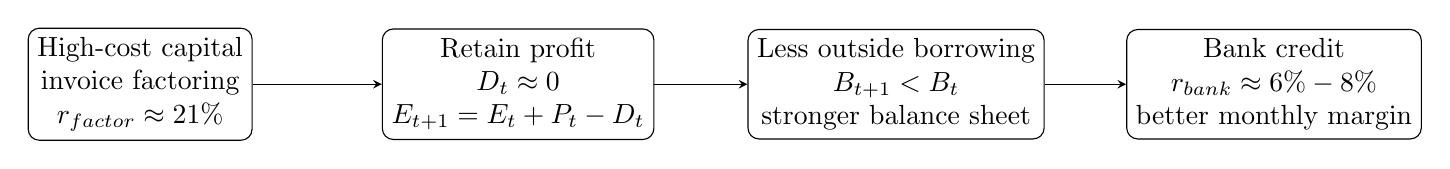
\begin{tikzpicture}[>=stealth]
\node[draw, rounded corners, align=center] (a) at (0,0) {High-cost capital\\invoice factoring\\\(r_{\text{factor}}\approx 21\%\)};
\node[draw, rounded corners, align=center] (b) at (4.8,0) {Retain profit\\\(D_t\approx 0\)\\\(E_{t+1}=E_t+P_t-D_t\)};
\node[draw, rounded corners, align=center] (c) at (9.6,0) {Less outside borrowing\\\(B_{t+1}<B_t\)\\stronger balance sheet};
\node[draw, rounded corners, align=center] (d) at (14.4,0) {Bank credit\\\(r_{\text{bank}}\approx 6\%-8\%\)\\better monthly margin};
\draw[->] (a.east) -- (b.west);
\draw[->] (b.east) -- (c.west);
\draw[->] (c.east) -- (d.west);
\end{tikzpicture}
\caption{Transcript reconstruction of the working-capital path described in the Ferrari interview.}
\end{figure}

The lecture also offers a monthly savings claim once financing costs fall. This invites a cautious back-of-the-envelope reconstruction.

\begin{remark}
The next computation is editorial. It is not spoken line by line in the interview; it merely converts the stated rate drop and the stated monthly savings into a rough implied capital base.
\end{remark}

Let \(K\) denote the average financed working-capital need, measured in millions of dollars, and let \(\Delta \Pi_{\text{month}}\) denote the improvement in monthly bottom line, also in millions. Then
\begin{align}
\Delta \Pi_{\text{month}} &\approx \frac{(r_{\text{factor}}-r_{\text{bank}})K}{12},\\
K &\approx \frac{12\,\Delta \Pi_{\text{month}}}{r_{\text{factor}}-r_{\text{bank}}}.
\end{align}
If we take the interview's monthly gain to be roughly \(0.02\) to \(0.025\) million dollars and the rate spread to be roughly \(0.13\) to \(0.15\), then \(K\) lies in the low seven figures. A representative midpoint gives
\begin{equation}
K \approx \frac{12\times 0.0225}{0.14}\approx 1.93,
\end{equation}
again measured in millions of dollars. We should not oversell this estimate, but it is a useful way to see what kind of working-capital burden the speaker is describing.

This, then, is the lecture's deepest financial chain:
\begin{enumerate}
\item expensive capital buys survival,
\item retained profit reduces dependence on that capital,
\item a stronger balance sheet makes cheaper capital available,
\item lower financing cost flows back into the monthly bottom line.
\end{enumerate}
The chapter should preserve this chain with great care, because it is where the lecture is most concrete.

\section{Passion, Refusal to Quit, and the Business of Medicine}

After the finance block, the Ferrari interview relaxes back into a more portable doctrine. The founder gives a two-part rule: find something one is truly passionate about, and do not quit. The lecture then briefly interrupts itself with a channel-community promotion before returning to a final interview with a doctor who owns a substantial medical business. This interruption should not dominate the notes, but it should not vanish entirely either; it is a marked pause before the last case study.

The doctor interview is important because it broadens the field. We are no longer speaking only about the founder of a high-growth firm. We are speaking about a physician who insists that the biggest mistake new doctors make is failing to learn the business of medicine.

In millions of dollars per year, the interview distinguishes professional earnings from business scale:
\begin{equation}
A_{\text{medicine}} \approx 0.6 \text{ to } 0.7,\qquad A_{\text{medical business}} \approx 6.
\end{equation}
The practice also carries a substantial payroll burden:
\begin{equation}
N_{\text{employees}} \approx 300.
\end{equation}

\subsection{Question \& Answer}

\paragraph{Question.} Why must even medicine be treated as a business system?

\paragraph{Answer.} The lecture's answer is not cynical. It does not say that medicine is merely a money game. It says something subtler: efficient care, solvency, payroll, and long-run survival are coupled. If the practice cannot stay afloat, then the doctor cannot sustainably care for patients at all.

\begin{remark}
This is one of the lecture's strongest closing moves. It does not reduce professionalism to money. It shows instead that a profession with moral content still requires operating competence, because cash-flow failure can destroy the institution in which the professional work is done.
\end{remark}

The doctor explicitly rejects the crude idea that one learns business in order to squeeze the system. Rather, one learns business in order to preserve a niche, pay staff, remain solvent, and keep attention on patients instead of on financial panic. In that sense the lecture ends where its finance material naturally points: business literacy is not ornament. It is a condition of durability.

\section{Summary}

The lecture begins with luxury objects and ends with operating logic. Its argument, once unfolded, is surprisingly tight. Refusal teaches persistence. The Texans interview turns persistence into cash conservatism, leverage, and the ability to walk away. The Ferrari interview turns organization into scale, then turns working capital into the central arithmetic of growth. The doctor interview shows that even a high-status profession eventually meets the same disciplines of efficiency, payroll, and solvency.

If we compress the chapter to its strongest internal spine, it is this: visible wealth is only the surface. Underneath it we find a small number of recurring rules --- do not quit, conserve cash, build organization, attach return to spend, retain profit when the firm is still fragile, and learn the business mechanics of one's field. The lecture never writes these principles on a board, but by the end they form a coherent notebook of their own.